\begin{figure}
    \centering
    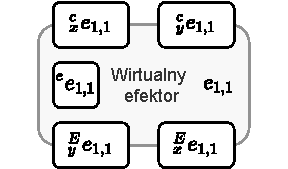
\includegraphics[width=0.75\columnwidth]{figures/ISR-ve-manip-model.pdf}
    \label{fig:model-vr-camera}
    \caption{Struktura ogólna wirtualnego efektora manipulatora sześciostopniowego}
\end{figure}

\begin{figure}
    \centering
    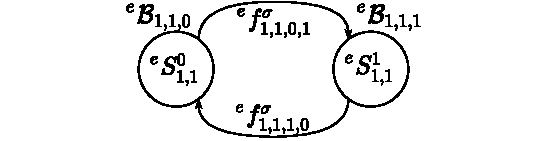
\includegraphics[width=\columnwidth]{figures/ISR-ve-manip-behaviours.pdf}
    \label{fig:zachowania-ve-manip}
    \caption{Automat zachowań wirtualnego efektora manipulatora sześciostopniowego}
\end{figure}

Zachowania:
\begin{itemize}
    \item ${}^{e}\mathcal{B}_{1,1,0}$ - idle,
    \item ${}^{e}\mathcal{B}_{1,1,1}$ - move.
\end{itemize}

Bufory komunikacyjne:
\begin{itemize}
    \item ${}^{c}_{x}e_{1,1} = \Theta_{\mathrm{zad}}$ - pozycja zadana we współrzędnych kartezjańskich,
    \item ${}^{c}_{y}e_{1,1} = \Theta$ - aktualna pozycja we współrzędnych kartezjańskich,
    \item ${}^{E}_{x}e_{1,1} = q$ - aktualna pozycja we współrzędnych konfiguracyjnych,
    \item ${}^{E}_{y}e_{1,1} = q_{\mathrm{zad}}$ - zadana pozycja we współrzędnych konfiguracyjnych,
    \item ${}^{e}e_{1,1} = [q_{\mathrm{ost}}, \Theta_{\mathrm{ost}}]$ - ostatnia znana pozycja we współrzędnych konfiguracyjnych oraz kartezjańskich.
\end{itemize}

Warunki początkowe:
\begin{itemize}
    \item ${}^{e}f^{\sigma}_{1,1,0} \triangleq \Theta_{\mathrm{zad}} \neq \Theta$,
    \item ${}^{e}f^{\sigma}_{1,1,1} \triangleq \Theta_{\mathrm{zad}} = \Theta$
\end{itemize}

Warunki końcowe:
\begin{itemize}
    \item ${}^{e}f^{\tau}_{1,1,0} \triangleq \Theta_{\mathrm{zad}} = \Theta$,
    \item ${}^{e}f^{\tau}_{1,1,1} \triangleq \Theta_{\mathrm{zad}} \neq \Theta$
\end{itemize}

Wymagane funkcje pomocnicze:
\begin{itemize}
    \item $FK(q)$ - kinematyka prosta, pozwala obliczyć pozycję końcówki robota w~przestrzeni kartezjańskiej, korzystając z~wiedzy na temat pozycji stawów robota,
    \item $IK(\Theta)$ - kinematyka odwrotna, pozwala obliczyć pozycję stawów, korzystając z~pozycji końcówki w~przestrzeni kartezjańskiej.
\end{itemize}

Funkcje przejścia w postaci matematycznej:
\begin{itemize}
    \item \textbf{idle} \begin{itemize}
        \item ${}^{e_{1,1}, E_{1,1}}f_{1,1,0} \triangleq {}^{E}_{y}e_{1,1} = q_{\mathrm{ost}}$,
        \item ${}^{e_{1,1}, c_{1,1}}f_{1,1,0} \triangleq {}^{c}_{y}e_{1,1} = \Theta_{\mathrm{ost}}$,
    \end{itemize} 
    \item \textbf{move} \begin{itemize}
        \item ${}^{e_{1,1}, E_{1,1}}f_{1,1,1} \triangleq {}^{E}_{y}e_{1,1} = IK(\Theta_{\mathrm{zad}})$
        \item ${}^{e_{1,1}, c_{1,1}}f_{1,1,1} \triangleq {}^{c}_{y}e_{1,1} = FK(q)$,
        \item ${}^{e_{1,1}, e_{1,1}}f_{1,1,1} \triangleq {}^{e}e_{1,1} = [q, FK(q)]$,
    \end{itemize}
\end{itemize}

\begin{figure}
    \centering
    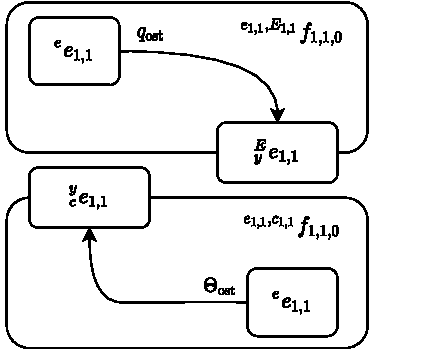
\includegraphics[width=\columnwidth]{figures/ISR-ve-manip-fp-idle.pdf}
    \label{fig:ve-manip-fp-idle}
    \caption{Zdekomponowana funkcja przejścia zachowania \textbf{idle} w~postaci DFD}
\end{figure}

\begin{figure}
    \centering
    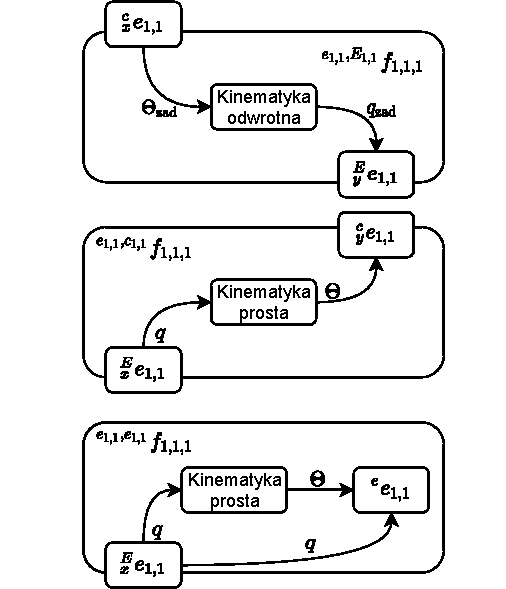
\includegraphics[width=\columnwidth]{figures/ISR-ve-manip-fp-move.pdf}
    \label{fig:ve-manip-fp-idle}
    \caption{Zdekomponowana funkcja przejścia zachowania \textbf{move} w~postaci DFD}
\end{figure}